\documentclass[10pt, xcolor=x11names]{beamer}
\usecolortheme{seagull}
\useoutertheme{infolines}
\usefonttheme[onlymath]{serif}
\setbeamertemplate{headline}[default]
\setbeamertemplate{navigation symbols}{}
\mode<beamer>{\setbeamertemplate{blocks}[rounded][shadow=true]}
\setbeamercovered{transparent}
\setbeamercolor{block body example}{fg=blue, bg=black!20}

\usepackage[utf8]{inputenc}
\usepackage[]{csquotes}
\usepackage{amsmath}
\usepackage{tikz, wasysym}
\usepackage{graphicx}
\usetikzlibrary{automata,positioning}
\usepackage{hyperref}
\usepackage{amsfonts}
\usepackage{csquotes}
\usepackage{tikz}
\usetikzlibrary{arrows}
\usetikzlibrary{arrows.meta}
\usepackage{wrapfig}
\usepackage{pgfplots}

%\usepackage{amsfonts}
%\usepackage{amssymb}
%\usepackage{makeidx}
%\usepackage{graphicx}


\usepackage{hyperref}
\author{Sven Fiergolla}
\title[Colloquium]{Improving Run Length Encoding through preprocessing}
\subtitle[short version]{}
\date{14. Januar 2020}
%\institute[Uni Trier]{Universität Trier}
%\logo{\includegraphics[scale=.25]{unilogo.pdf}}

\begin{document}
	\frame{\maketitle}
	\frame{\frametitle{}
	\tableofcontents
	}



\section{Introduction}	
\frame{\frametitle{Introduction - A Bit of History}
	  \begin{itemize}
		\item rise of multimedia
		\item rise of the World Wide Web
		\item ever increasing data transfer
	\end{itemize}

\medskip 

  \begin{itemize}
	\pause \item compress to save storage space \& to handle new types and volumes of data
\end{itemize}	
}

\frame{\frametitle{Introduction - The Situation Today}
	\begin{itemize}
		\item burst of sensors and IoT
		\item massive and rapid increasing data transfer
	\end{itemize}
	
	\medskip 
	
	\begin{itemize}
		\pause \item compress to lower transmission cost / time
		\item compress to handle increasing resolution, fidelity, dynamic range
		\item compression for cold archiving
	\end{itemize}	
}

\section{Basics}
\frame{\frametitle{Basics of Compression}
	\begin{itemize}
		\item Non random data contains redundant information
		\item Compression is about pattern or structure identification and exploitation
		\pause \item No algorithm can compress all possible data of a given length, even by one byte (Kolmogorov Complexity)
	\end{itemize}	
}

\frame{\frametitle{Huffman Encoding}
\begin{figure}[h]
	\centering
	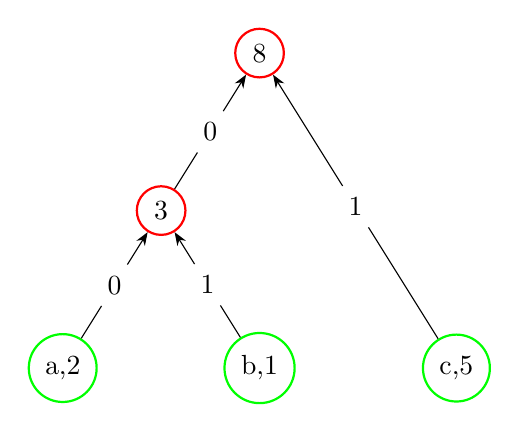
\begin{tikzpicture}
	\begin{scope}[every node/.style={circle,thick,draw=red}]
	\visible<2->{\node (B) at (1.25,2) {3};}
	\visible<3->{\node (C) at (2.5,4) {8};}
	\end{scope}
	\begin{scope}[every node/.style={circle,thick,draw=green}]
	\node (A) at (0,0) {a,2};
	\node (D) at (2.5,0) {b,1};
	\node (F) at (5,0) {c,5} ;
	\end{scope}
	
	\begin{scope}[>={Stealth[black]},
	every node/.style={fill=white,circle}]
	\visible<2->{\path [->] (A) edge node {$0$} (B);}
	\visible<3->{\path [->] (B) edge node {$0$} (C);}
	\visible<2->{\path [->] (D) edge node {$1$} (B);}
	\visible<3->{\path [->] (F) edge node {$1$} (C);}
	
	\end{scope}
	\end{tikzpicture}
	\caption{Example Huffman tree with 3 leaf nodes.} \label{fig:M1:example Huffman tree}
\end{figure}
}

\section{Design}
\frame{\frametitle{Design}

}
\section{Analysis}
\frame{\frametitle{Analysis}
	
}
\section{Implementation}
\frame{\frametitle{Implementation}
	
}
\section{Evaluation and Discussion}
\frame{\frametitle{Evaluation and Discussion}
	
}
\end{document}
